\chapter{Обзор системы} \label{overview}

Рисунок~\ref{fig:overview} показывает главные компоненты поддержки отладки.
Блоки, обозначенные пунктиром, являются опциональными.

\begin{figure}
   \centering
   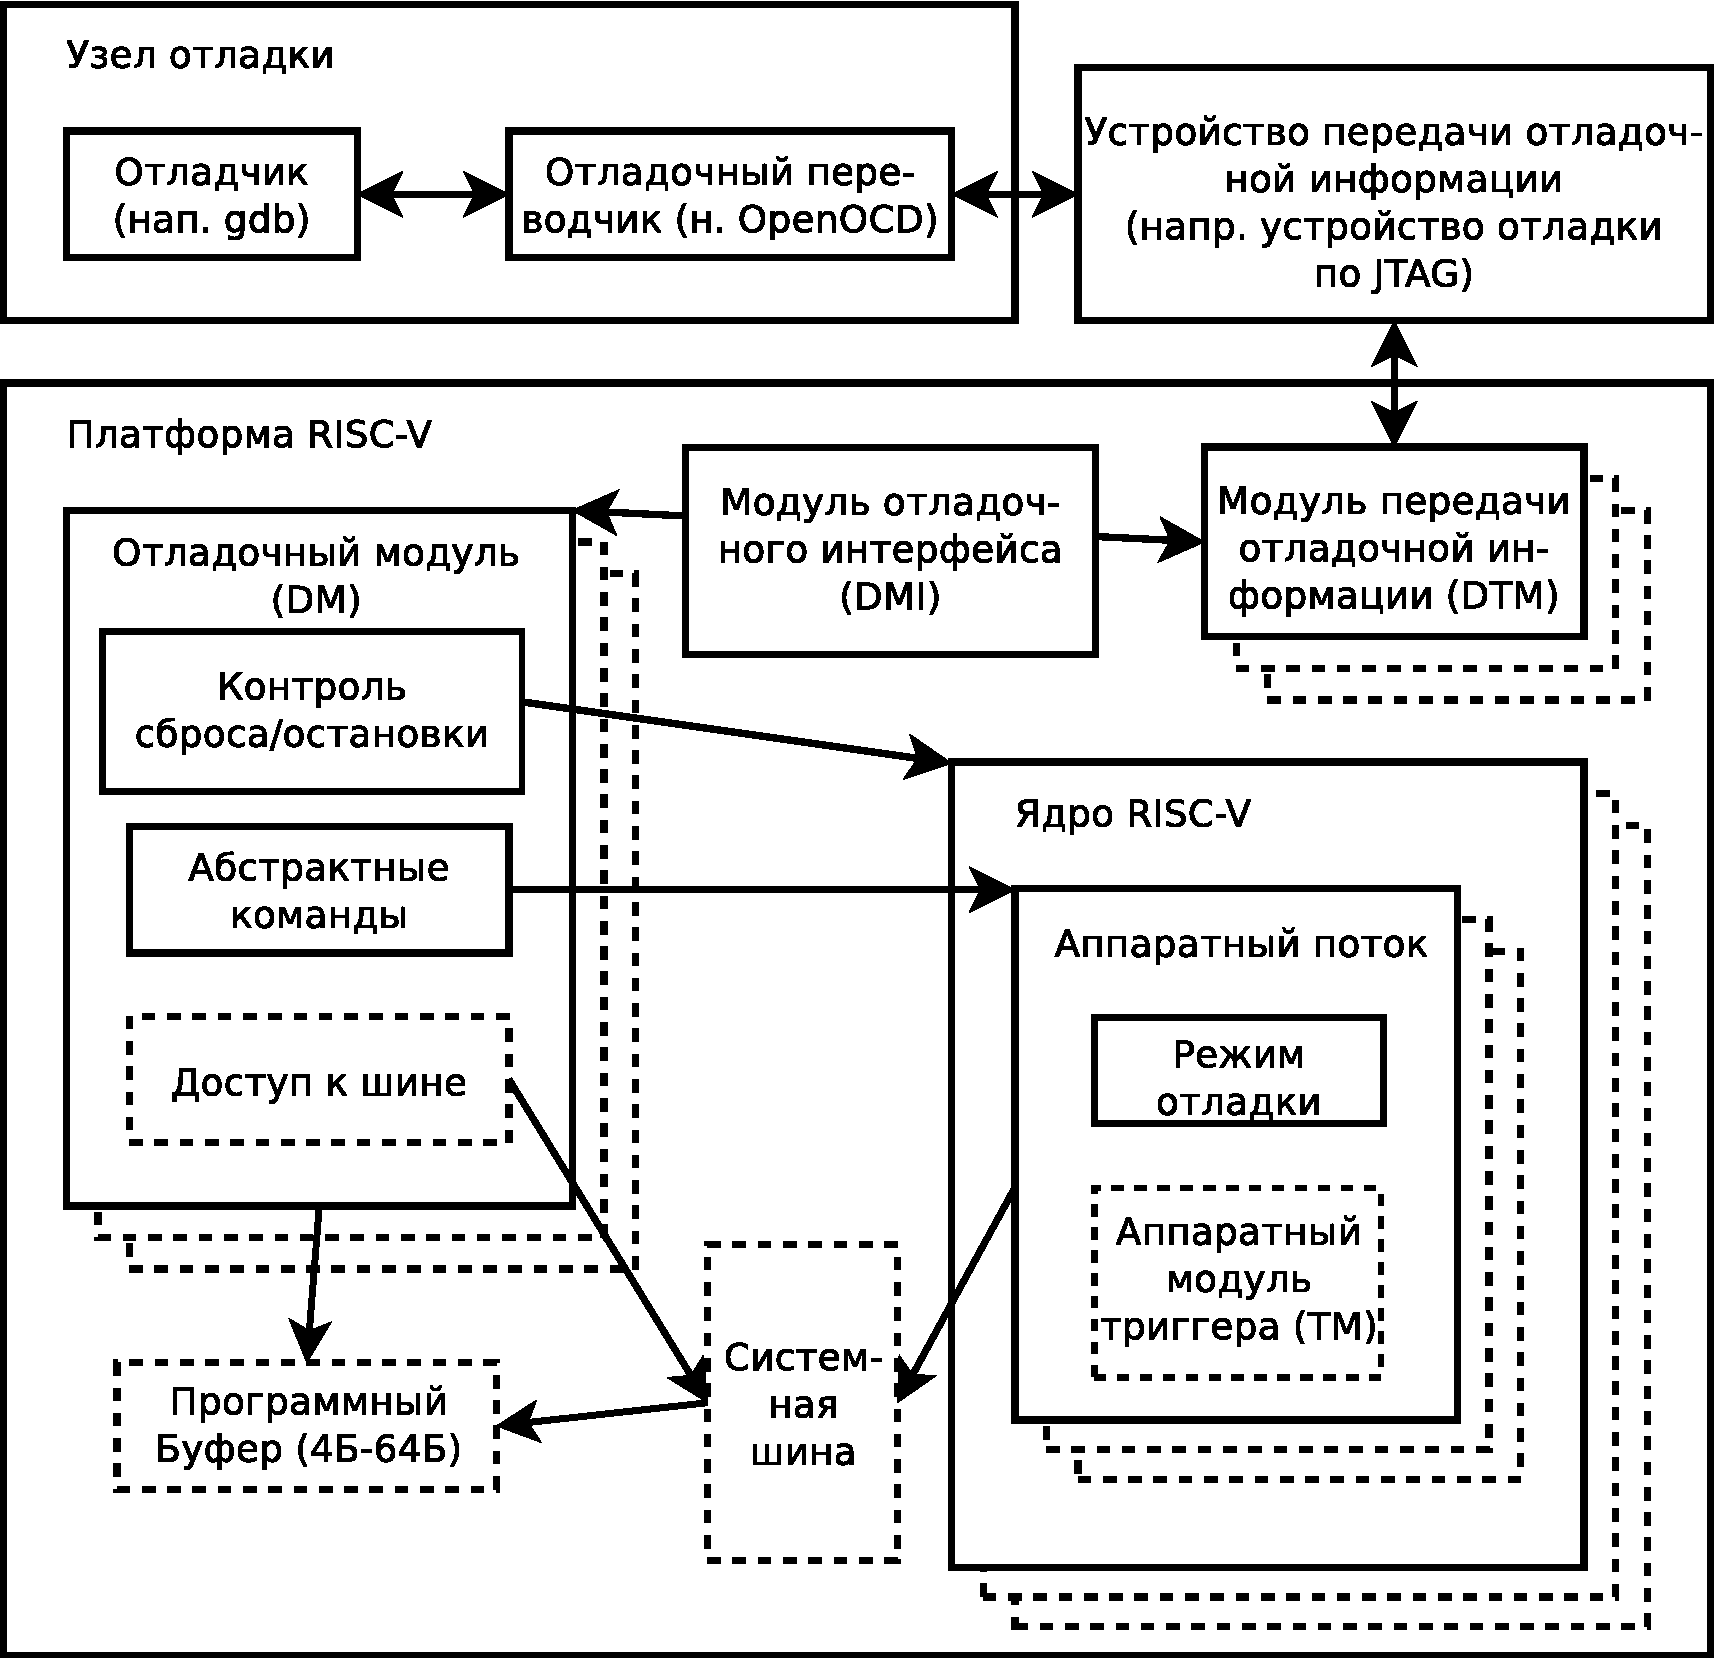
\includegraphics[width=\textwidth]{fig/overview-eps-converted-to.pdf}
   \caption{Обзор системы отладки в RISC-V}
   \label{fig:overview}
\end{figure}

Пользователь взаимодействует с узлом отладки (например ноутбуком), на котором
запущен отладчик (например gdb). Отладчик работает с отладочным переводчиком
(например OpenOCD, к которому может быть подключён аппаратный драйвер) для связи 
с устройством передачи отладочной информации (например Olimex USB-JTAG adapter).
Данное устройство подключает узел отладки к DTM аппаратной платформы.
DTM предоставляет доступ к одному или нескольким DM, используя DMI.

Каждый hart в аппаратной платформе управляется только одним DM. Hart-ы могут быть
гетерогенными. Лимита по ассоциации hart-ов с DM не существует, но обычно
все hart-ы в пределах одного ядра управляются одним и тем же DM. В большинстве аппаратных платформ
будет только один DM, управляющий всеми hart-ами в аппаратной платформе.

DM-ы предоставляют контроль запуска их hart-ов в аппаратной платформе. Абстрактные команды
дают доступ GPR-ам. Дополнительные регистры доступны через абстрактные команды или запись
программ в опциональный программный буфер.

Программный буфер позволяет отладчику запускать произвольные инструкции на
hart-е. Этот механизм также может использовать память. Необязательный блок доступа
к системной шине допускает доступ к памяти без использования для этих целей hart-а RISC-V.

Каждый hart RISC-V может реализовывать TM. Когда выполнены условия триггера,
hart-ы остановятся и проинформируют DM о своей остановке.
